\documentclass[lualatex]{beamer}

\usepackage{fontspec}
\usepackage{fancyvrb}
\usefonttheme{professionalfonts}%  don't change fonts inside beamer
\setmainfont{Lucida Grande}
\setsansfont{Lucida Grande}
\usepackage{unicode-math}
\setmathfont{Asana Math}

\author{Jesper Louis Andersen\\jesper.louis.andersen@gmail.com\\Shopgun Aps}
\date{\today{}}
\title{Real World QuickCheck\\DTU}

\begin{document}

\maketitle

\begin{frame}
\frametitle{Who is Jesper?}
\begin{itemize}
\item Functional programming, type theory, semantics
\item 10 years of Erlang experience
\item 5+ years with QuickCheck
\item Works for a small startup, ShopGun Aps.,
\item BA in CS from Copenhagen University
\end{itemize}
\end{frame}

\begin{frame}
\frametitle{Erlang — in one slide}
Erlang is an (untyped) functional language, with three main focal points:
\begin{itemize}
\item Communication—Concurrency, Protocol handling
\item Robustness—Self-healing, Hardware failure tolerance, soft-realtime
\item Continuous operation—Hot code loading, late binding, dynamic reconfiguration
\end{itemize}

Built originally for telecommunications, in 1986.

Most of the Erlang in this talk is by osmosis.
\end{frame}

\begin{frame}[fragile]
\frametitle{QuickCheck — summary}
We would like to prove a property, such as
\begin{equation}
\begin{split}
	\forall a \in \text{array}(byte) :\\
	\quad \quad unzip(zip(a)) = a
\end{split}
\end{equation}
\begin{itemize}
\item Proof—requires lemmas and theorems about \emph{zip/unzip}, exploiting their structure
\item Check all arrays up to size $n$ is extremely time-consuming, even on large clusters
\item Quickcheck—Generate samples of $a$ via highly skewed distributions
\end{itemize}
\end{frame}

\begin{frame}[fragile]
\frametitle{QuickCheck - summary}
Erlang QuickCheck notation for the example would be:
\begin{verbatim}
prop_zip_inverse() ->
    ?FORALL(Arr, list(choose(0, 255)),
        begin
            Bin = list_to_binary(Arr),
            Z = zlib:uncompress(zlib:compress(Bin)),
            measure(array_length, length(Arr),
                equals(Bin, Z))
        end).
\end{verbatim}
Example output:
\begin{verbatim}
prop_zip_inverse: … OK, passed 100 tests
array_length:
    Count: 100   Min: 0   Max: 10   Avg: 2.850
    StdDev: 2.350   Total: 285
\end{verbatim}
\end{frame}

\begin{frame}[fragile]
\frametitle{QuickCheck - summary}
``Program testing can be used to show the presence of bugs, but never to show their absence!'' — Dikjstra EWD249 1970

\begin{itemize}
\item Do \emph{not} generate a uniform distribution.
\item Use heuristics and target where the needle/bug is most likely to be in the haystack
\item Generate the nastiest examples which are unlikely to occur in normal operation
\item Once a counterexample is found, employ a \emph{shrinking} strategy to search for a smaller one
\item The power stems from statistical amplification and turning clock cycles into error-finding
\end{itemize}

Doing this well is (part of) the secret, which is the intellectual property of e.g., Quviq's commercial ``Erlang QuickCheck'' implementation.
\end{frame}

\begin{frame}[fragile]
  \frametitle{Story}
  Around 10 years ago (2007), a major change in software development started:
  \begin{description}
  \item[Virtualization] Fractional hardware
  \item[Leasing/Elasticity] You don't own the machine
  \item[Containerization] Standardized components
  \end{description}
\end{frame}

\begin{frame}
  \frametitle{Problem statement}
  \begin{itemize}
  \item Systems are now scattered over multiple machines
  \item Highly distributed
  \item You don't control the lifetime of systems(!)
  \item Must cope with the problem of cascading failures in components
    with dependencies:
  \end{itemize}
  \begin{equation}
    \label{eq:1}
    A \to B \to C
  \end{equation}
  If $C$ fails, then resource buildup happens on $B$ due to timeouts. Once $B$ fails,
  cascades to $A$
\end{frame}

\begin{frame}
  \frametitle{Blame management}
  \begin{itemize}
  \item Under cascading failure, often the wrong component is blamed
  \item Think it is $A$ or $B$ while the underlying problem is $C$
  \item Takes debugging time, often in production
  \end{itemize}
\end{frame}

\begin{frame}
  \begin{itemize}
  \item A ``circuit breaker'' is a pattern (Michael Nygard, Release
    It! 2007)
  \item Imagine a very big off-switch
  \item If a component is failing too often, hit the switch
  \item After a while try to re-enable the failed component
  \end{itemize}
\end{frame}
\begin{frame}
  Consequence:
  \begin{itemize}
  \item Turn timeouts into fast errors
  \item No resource buildup
  \item Better response times (close to a couple microseconds)
  \item A client knows only about itself, the circuit has holistic
    knowledge
  \item Give the failing component a break so it can recover from
    transient errors
  \item Monitoring of broken circuits places blame accurately
  \end{itemize}
\end{frame}

\begin{frame}
  \frametitle{Our problem}
  \begin{itemize}
  \item Major outages due to failing cascades
  \item Want graceful degrade of system
  \item We had no direct control over all components, so it was not
    possible to fix all of them
  \end{itemize}
\end{frame}

\begin{frame}[fragile]
  \frametitle{Solution}
  Build an Erlang component, \texttt{fuse}, for handling circuit breaking:
\begin{verbatim}
Configuration = ...,
fuse:install(Name, Configuration)

case fuse:ask(Name) of
    ok ->
        normal_operation;
    blown ->
        return_error
end

%% When a system fails
ok = fuse:melt(Name)
\end{verbatim}
\end{frame}

\begin{frame}[fragile]
  \frametitle{Example}
  \begin{itemize}
  \item A configured policy defines how many errors to tolerate
  \item Policy configures when to try re-enabling the circuit again
  \item Decouples policy from implementation and the protected
    component
  \item Policy code is not on the fast-path: better latency and
    efficiency of the system
  \end{itemize}
\end{frame}

\begin{frame}
  \frametitle{Robustness}
  \begin{itemize}
  \item Circuit breakers are critical components
  \item If there is a bug in the breaker, then the system is less
    robust overall
  \item In Erlang programming we say that it is part of the ``error
    kernel'' - the part of the system which absolutely must be correct
    for correct operation
  \item General robustness principle: trust few components. Use them
    to make the rest of the system robust
  \end{itemize}
\end{frame}

\begin{frame}
  \frametitle{QuickCheck!}
  \begin{itemize}
  \item Cost/Benefit analysis makes core components highly eligible
    for more extensive testing.
  \item QuickCheck is an excellent light-weight formal method: for
    relatively little work, you gain lots of robustness in the system
  \item Implementation time is roughly 3-5 times normal development
  \item But components have almost no maintenance afterwards
  \end{itemize}
\end{frame}

\begin{frame}
  \frametitle{Strategy}
  Build software like the 'Dogme 95' manifesto for movies:
  \begin{itemize}
  \item Write the model in QuickCheck \emph{first}
  \item Then write the code for the system
  \item Any feature must have a main user and use case (dogfood
    principle)
  \item If you can't specify the model, the feature is not going in
  \end{itemize}
\end{frame}

\begin{frame}
  \frametitle{Result}
  \begin{itemize}
  \item One minor bug in 3 years of operation
  \item Almost no reported issues
  \item Almost no maintenance
  \item The model is a specification
  \item Documentation is far easier to write with a good specification
  \item Extremely small code base
  \item Many bugs caught early on, when they are cheap to fix
  \end{itemize}
\end{frame}

\begin{frame}
  \frametitle{Approach: first version}
  \begin{itemize}
  \item Stateful model
  \item The major commands of a fuse is modeled (install, ask, melt)
  \item Pick a static configuration, and keep it simple (1 failure
    allowed in a 60 second window)
  \item Once the static configuration works, extend the code to
    arbitrary configurations
  \item Then implement minor commands (reset, remove)
  \end{itemize}
\end{frame}

\begin{frame}
  \frametitle{Whiteboard time}
\end{frame}

\begin{frame}[fragile]
\begin{verbatim}
%% Manual reset
reset(Name) ->
    fuse:reset(Name).

reset_pre(S) ->
    has_fuses_installed(S).

reset_args(_S) ->
    [g_name()].

%% (Postcondition)
reset_return(S, [Name]) ->
    case is_installed(Name, S) of
        true -> ok;
        false -> {error, not_found}
    end.
\end{verbatim}
\end{frame}

\begin{frame}[fragile]
\begin{verbatim}
%% Resetting a fuse resets its internal state
reset_next(S, _V, [Name]) ->
    case is_installed(Name, S) of
        false -> S;
        true ->
          clear_blown(Name,
            clear_melts(Name,
              S))
     end.

reset_features(S, [Name], _V) ->
    case is_installed(Name, S) of
        false -> [{fuse_eqc, r05,
                   reset_uninstalled_fuse}];
        true -> [{fuse_eqc, r06,
                   reset_installed,
                      {blown, is_blown(Name, S)}}]
    end.
\end{verbatim}
\end{frame}

\begin{frame}[fragile]
  \frametitle{Feature sets}
\begin{verbatim}
    Group heal:
    R01 - Heal non-installed fuse
    R02 - Heal installed fuse

    Group install:
    R03 - Installation of a fuse with invalid conf
    R04 - Installation of a fuse with valid conf

    Group Reset:
    R05 - Reset of an uninstalled fuse
    R06 - Reset of an installed fuse
\end{verbatim}
\end{frame}

\begin{frame}
  \frametitle{Approach: second version}
  \begin{itemize}
  \item Stateful model, parallel version
  \item Ask Erlang QuickCheck to run the model in parallel with
    multiple clients asking at the same time
  \item One-line code change for this to happen(!)
  \item 1. Run the model sequentially up to a point
  \item 2. Run the model in parallel from this point on
  \item 3. Look for a linearization: If we can't find one, the code
    is wrong
  \end{itemize}
\end{frame}

\begin{frame}
  \frametitle{Approach: third version}
  \begin{itemize}
  \item Stateful model, parallel, PULSE
  \item Parallel test cases are hard to shrink
  \item Usually the error does not reappear under shrinking
  \item PULSE allows us to control the parallel \emph{schedule} of the
    system
  \item Thus we can keep the bad interleave of concurrency while
    shrinking
  \item Uncovered an asynchronous bug in the system
  \end{itemize}
\end{frame}

\begin{frame}[fragile]
  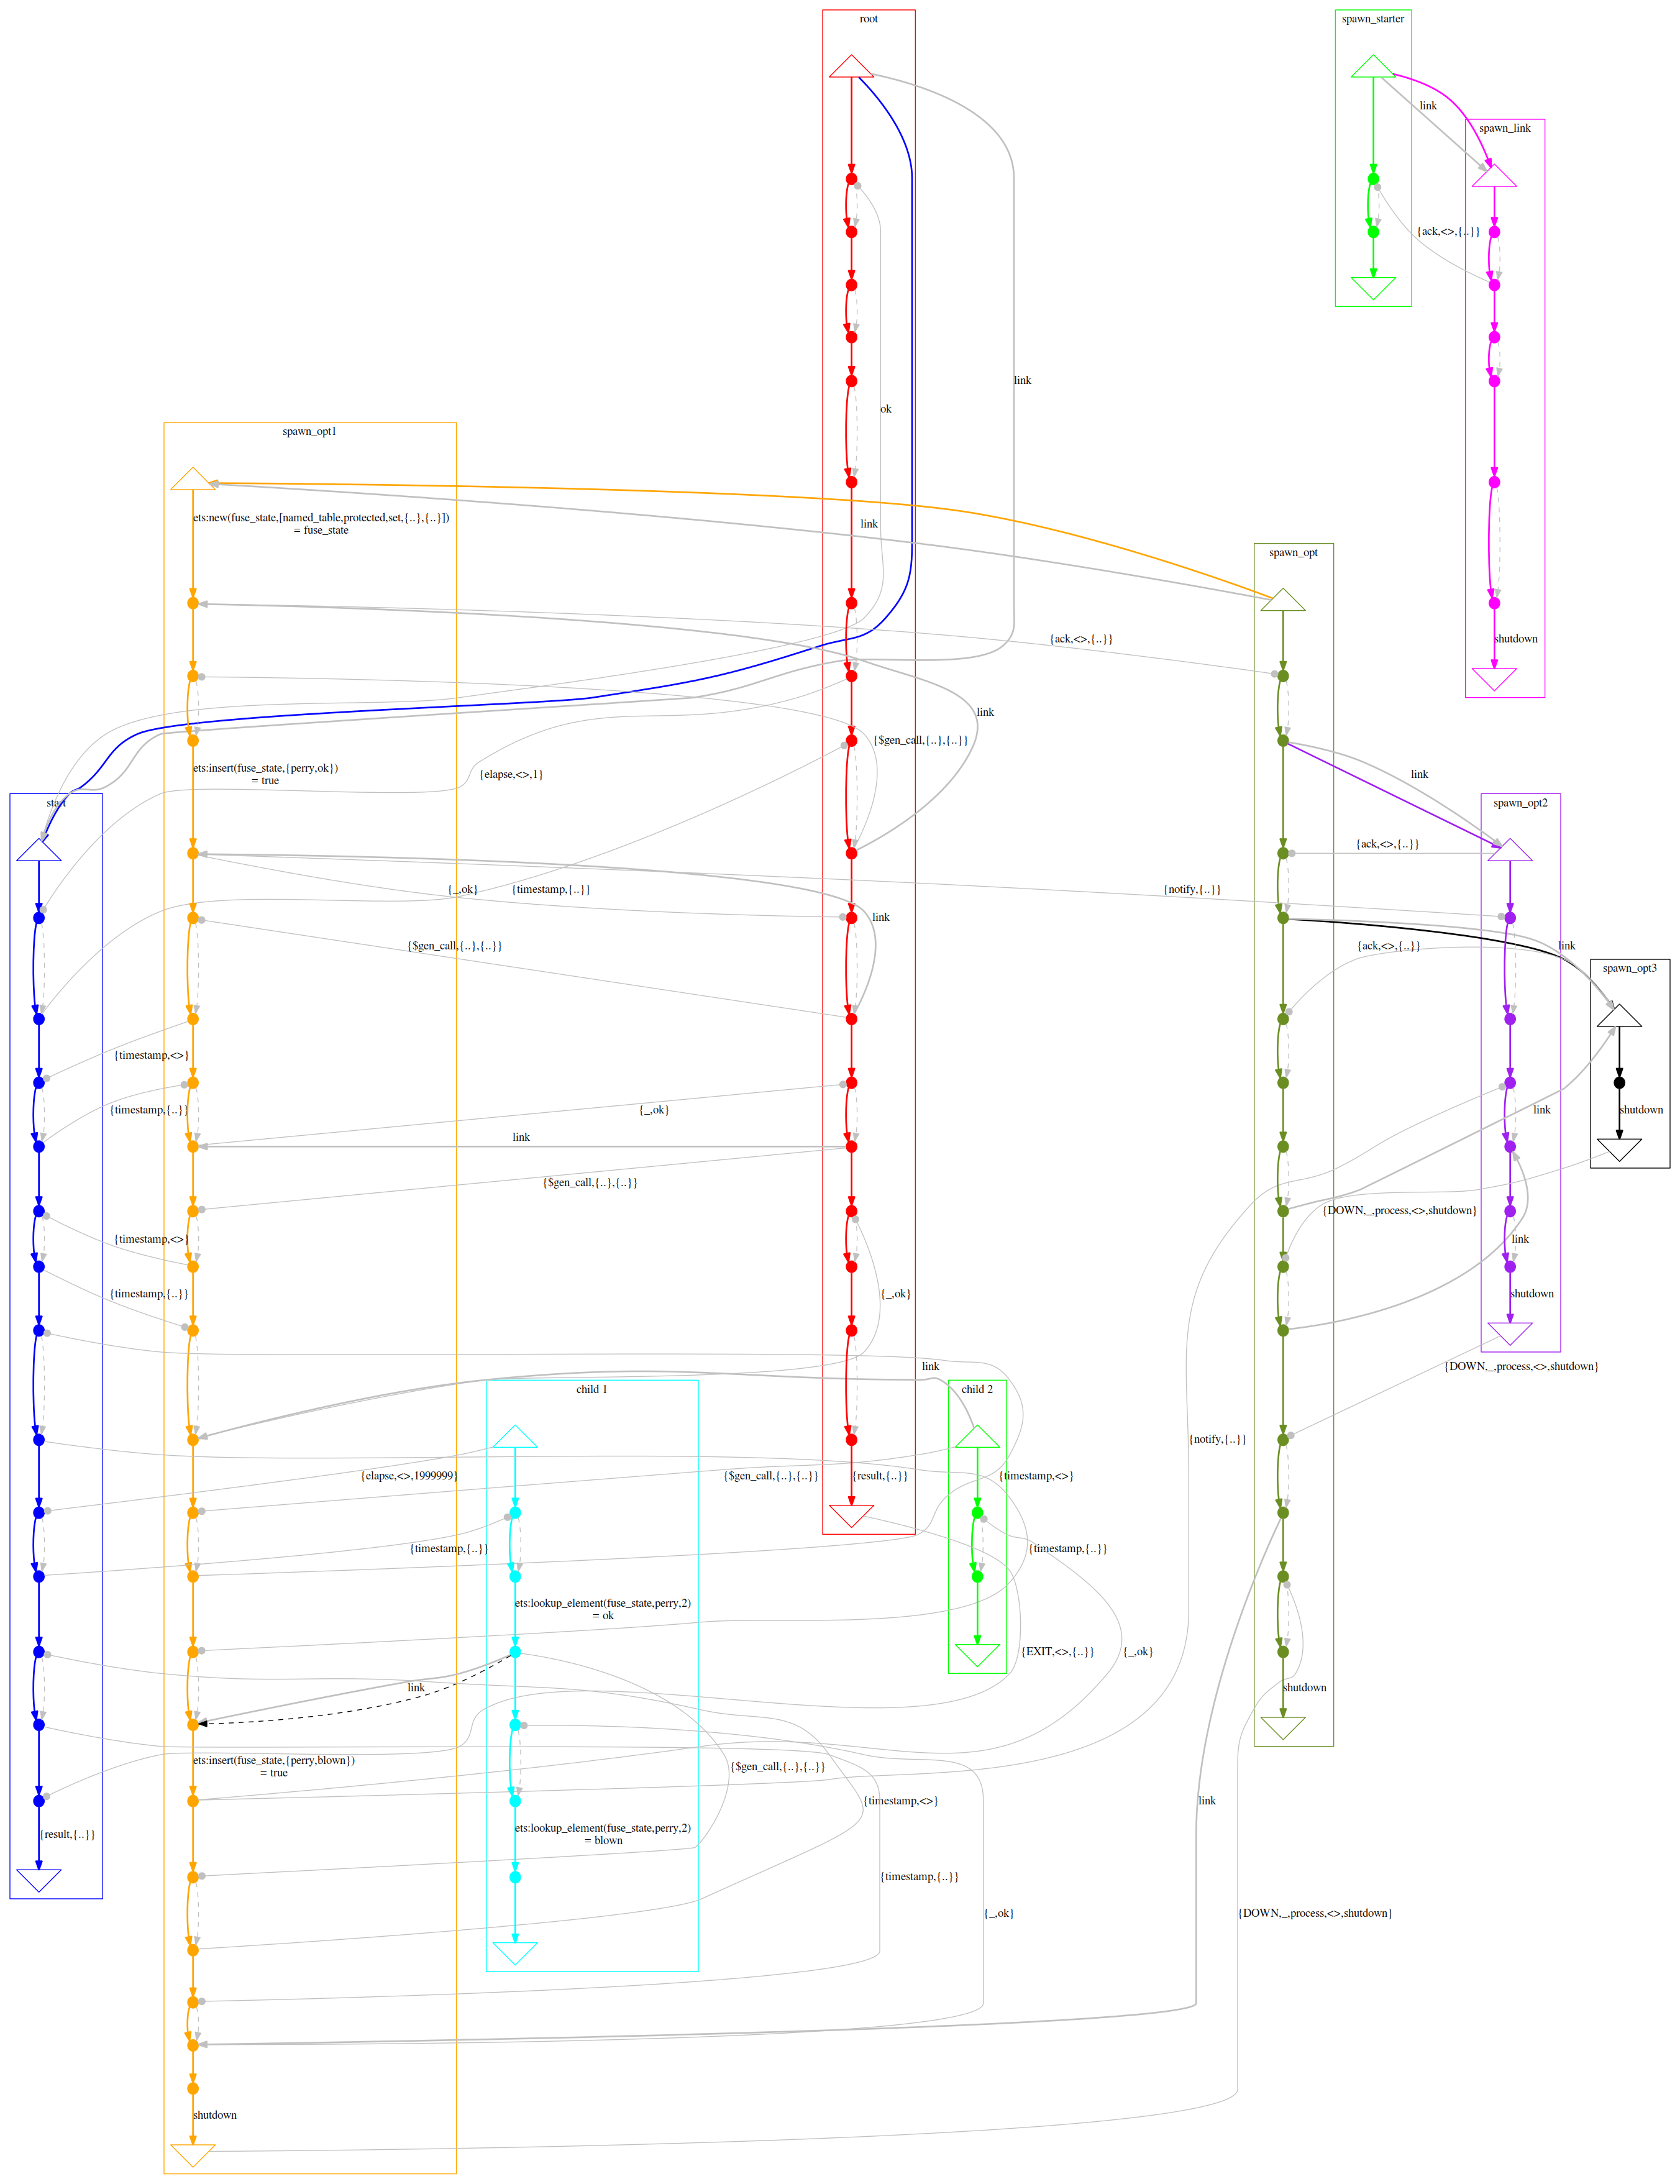
\includegraphics[scale=0.1]{pulse_output.png}
\end{frame}

\begin{frame}
  \frametitle{Approach: Current Version}
  \begin{itemize}
  \item Clustered Component model
  \item 2 stateful models: one handles fuse, the other handles time
  \item Clustered into a complete system
  \item Time and timers are \emph{mocked} - taken over by the model
  \item Advancing of time is controlled by the model and simulated
  \item Allows us to efficiently check timing related questions
  \end{itemize}
  Time injection is a key trick in most real-world-systems!
\end{frame}

\begin{frame}
  \frametitle{Mocking}
  \begin{itemize}
  \item In addition to checking postconditions of the system:
  \item Check that the system calls the correct functions in a callout
    section
  \item Domain-specific-language for defining callout sequences and
    verifying their correctness
  \end{itemize}
\end{frame}

\begin{frame}
  \frametitle{Clusters}
  \begin{itemize}
  \item 2 Stateful models
  \item We can invoke commands in either model: either for advancing
    time, or for doing some command in fuse
  \item fuse calls \emph{into} the timing model whenever it needs time
    or timing information
  \item We construct answers from the timing model to feed back into
    fuse
  \item We can do model-internal transitions: Change the state of the
    model without invoking a command in the system-under-test
  \end{itemize}
\end{frame}

  
\begin{frame}[fragile]
  In the timing module:
  \begin{verbatim}
monotonic_time_callouts(#state {time = T }, []) ->
  ?CALLOUT(fuse_time, monotonic_time, [], T),
  ?RET(T).

monotonic_time_return(#state { time = T }, []) -> T.
  \end{verbatim}
\end{frame}

\begin{frame}[fragile]
  In the fuse model:
  \begin{verbatim}
melt_installed_callouts(_S, [Name]) ->
    ?MATCH(Ts, ?APPLY(fuse_time_eqc, monotonic_time, [])),
    ?APPLY(process_melt, [Name, Ts]),
    ?RET(ok).
\end{verbatim}
  \begin{itemize}
  \item Apply the operations of another module
  \item Apply a \emph{model-internal} transition in \texttt{process\_melt}
  \end{itemize}
  (For the Haskell-nerds in the room: callouts is a monad)
\end{frame}

\begin{frame}
  \frametitle{Errors found}

  \begin{itemize}
  \item Under development 15 errors were removed
  \item The model was guiding the implementation along, suggested
    better approaches
  \item The model forces you into simple, coherent solutions
  \end{itemize}
\end{frame}

\begin{frame}
  \frametitle{Use}
  \begin{itemize}
  \item Used in various industries around the world:
  \item Game servers
  \item Ad Tracking services
  \item Ad bidding services
  \item Database systems
  \item Some very big corporations are using it (top 10)
  \end{itemize}
\end{frame}
\end{document}
